\documentclass[tikz,border=6pt]{standalone}
\usepackage[T1]{fontenc}
\usepackage[utf8]{inputenc}
\usepackage{amsmath,amssymb}
\usepackage{tikz}
\usetikzlibrary{automata,positioning,arrows.meta,shapes.geometric,calc,fit}
\tikzset{
    >=Stealth,
    every state/.style={minimum size=8mm, inner sep=1pt, font=\small},
    flow/.style={rectangle, rounded corners, draw, align=center, minimum width=3.1cm, minimum height=0.9cm},
    decision/.style={diamond, draw, aspect=2.0, align=center, inner sep=1.5pt},
    terminal/.style={ellipse, draw, align=center, minimum width=2.4cm, minimum height=0.85cm},
    module/.style={rectangle, draw, rounded corners, align=center, minimum width=3.4cm, minimum height=1.0cm},
    data/.style={rectangle, draw, align=center, minimum width=3.2cm, minimum height=0.9cm}
}
\begin{document}
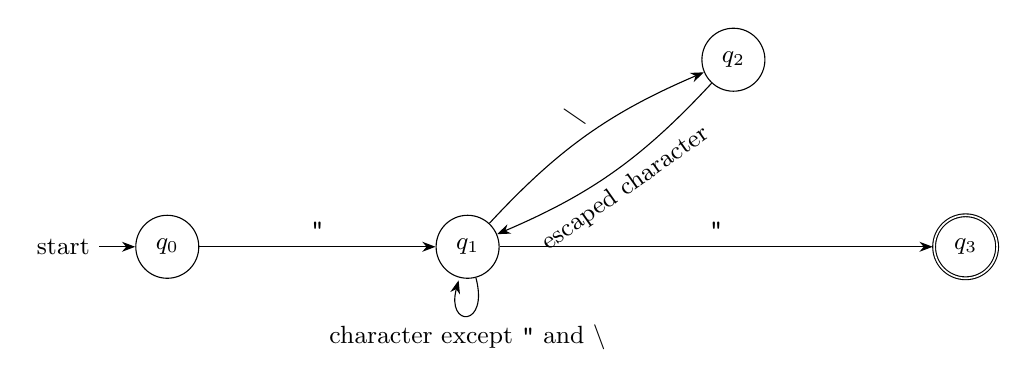
\begin{tikzpicture}[->, node distance=30mm, font=\small]
    \node[state, initial] (q0) {$q_0$};
    \node[state, right=of q0] (q1) {$q_1$};
    \node[state, above right=18mm and 28mm of q1] (q2) {$q_2$};
    \node[state, accepting, right=55mm of q1] (q3) {$q_3$};

    \path (q0) edge node[above] {\texttt{"}} (q1)
          (q1) edge[loop below] node {character except \texttt{"} and \textbackslash} (q1)
          (q1) edge[bend left=12] node[above,sloped] {\textbackslash} (q2)
          (q2) edge[bend left=12] node[below,sloped] {escaped character} (q1)
          (q1) edge node[above] {\texttt{"}} (q3);
\end{tikzpicture}
\end{document}
